\documentclass[11pt, a4paper]{article}
\usepackage[utf8]{inputenc}
\usepackage{fullpage}
\usepackage{graphicx}
\usepackage{markdown}
\usepackage[hidelinks]{hyperref,xcolor}
\renewcommand\UrlFont{\color{blue}\rmfamily}

\usepackage[backend=biber]{biblatex}
\addbibresource{library.bib}
\title{Project Plan\\Remote Water Sensing using UAVs}
\author{Robin \textsc{Westerik}}

\newcommand{\supervisors}{Jan \textsc{Bollen}\\Harry \textsc{Futselaar}}
\newcommand{\timePeriod}{February 2022 - June 2022}
\newcommand{\resourcesPlanned}{800 hours (40h per week)}
\newcommand{\homepage}{\url{https://github.com/organizations/remotewatersensing/}}
\date{\today}

\makeatletter{}

\begin{document}

\begin{titlepage}
  	\newcommand{\HRule}{\rule{\linewidth}{0.3mm}}
	\center
	\textsc{\LARGE Saxion University of Applied Sciences}\\[1.5cm]
	\textsc{\Large International Water Technology}\\[0.5cm]
	\textsc{\large Applied Computer Science Graduation Project}\\[0.5cm]
	\HRule\\[0.4cm]
	{\huge\bfseries \@title}\\[0.4cm]
	\HRule\\[1.5cm]

	%Author(s)
	\begin{minipage}{0.4\textwidth}
		\begin{flushleft}
			\large
			\textit{Author(s)}\\
			\@author % Your name
		\end{flushleft}
	\end{minipage}
	~
	\begin{minipage}{0.4\textwidth}
		\begin{flushright}
			%\large
			%\textit{Supervisor(s)}\\
			%\supervisors
		\end{flushright}
	\end{minipage}
	
% 	If you don't want a supervisor, uncomment the two lines below and comment the code above
% 	{\large\textit{Author(s)}}\\
% 	\@author % Your name

	%Date
	\vfill\vfill
		{\large\today}
    \vfill\vfill
    
    \footnotesize{Time period: \timePeriod}
    \\[0.3cm]
    \footnotesize{Resources planned: \resourcesPlanned}
    \vfill
    \homepage
    
    \vfill
    
    \begin{tabular}{ | l | l | l | l |}
    \hline
    \textbf{Version} & \textbf{Date of change} & \textbf{What is changed?} & \textbf{The reason for the change} \\ \hline
    0.1 & 03-02-2022 & templating & \\
    0.2 & 03-02-2022 & added project result & \\
    0.21 & 07-02-2022 & edited project result & added research question\\
    0.3 & 07-02-2022 & added project activities &\\
    0.4 & 07-02-2022 & added project boundaries &\\
    0.5 & 08-02-2022 & added interim results, quality &\\
    \hline
\end{tabular}
	
	\vfill\vfill
	
\includegraphics[width=0.4\textwidth]{./saxionlogo.png}
	\vfill
	 
	\vfill
	
\end{titlepage}


\tableofcontents
\pagebreak

\section{Background}
This project proposal has been brought forward by an idea of the International Water Technology lectorate at the Saxion University of Applied Sciences. The project will be carried out in collaboration with PERNAM JSC. Ton Duc Thang University will further accommodate the project when possible by providing expert advice and practical necessities. As this project will be a first of potential following projects, emphasis is laid on developing an open source and well documented foundation so that future parties can build on this project in the future. 

Completing this project could be a start of providing smarter water sensing solutions which in turn could benefit current water filtration solutions of PERNAM as well as help with several water availability issues.

\subsection{PERNAM JSC}
PERNAM JSC \cite{pernam} is an engineering firm specializing in water treatment solutions in Vietnam. They are specialized in the design, engineering, and construction supervision of water treatment technologies for groundwater, surface, and brackish water. The company partially originated from the Netherlands and has close connections with Vitens, the biggest water supply company in the Netherlands. PERNAM is closely related to Howaco, the only private water supply company who is member of the South Vietnam VWSA.

\subsection{Ton Duc Thang University}
TDTU \cite{tdtu} is a public research university with the main campus in Ho Chi Minh City, Vietnam. The University offers 40 undergraduate programs, 18 master programs and 25 doctoral programs in variety of areas such as: law, applied science, technology, vocational skills, social sciences, economics, business, foreign languages and arts. 

\subsection{Mekong Delta}
This project will be focused around the Mekong Delta. The Mekong Delta is a network of tributaries in southwest Vietnam, between Ho Chi Minh City and Cambodia. The river itself starts in the Himalayas and passes through China, Myanmar, Thailand and Cambodia before reaching Vietnam.

The Mekong Delta is generally regarded as vital to the Vietnamese economy: A fourth of Vietnam's total agricultural sector takes place in the Mekong Delta. It is also regarded as Vietnam's most important fishing region, contributing more than half of Vietnam's total fishery output \cite{vietstats}

The region's production capabilities is threatened by multiple external sources. Vietnam has little influence on the water levels of the Mekong River, because the amount of water flowing into the country is regulated by dams in China and Laos. The quality of the water also differs regularly because of these upstream influences. Climate change also plays a big part, with more rainy seasons and a rise of sea levels. \cite{wur}

Apart from external influences, the Mekong Delta is also rapidly losing elevation due to accelerating subsidence rates, primarily caused by increasing ground water extraction. This strongly increases the delta’s vulnerability to flooding, salinization, and coastal erosion. \cite{minderhoud2020}
\pagebreak
\section{The Project}
Intelligent surface water treatment can be a valuable asset to reduce the need for ground water extraction. A typical challenge of surface water treatment is determining the quality of the input water. The objective during this graduation project is to explore new ways in which this water can be autonomously monitored in local, remote, and harder to measure locations. Specifically, this project will be taking a look at the use of unmanned aerial vehicles (drones) to do this task. 

While it is not possible to know in advance exactly what the end product would entail, it would allow users to measure various water quality variables across an area by using unmanned aerial vehicles and various different water quality sensor concepts. Future projects could mature by for example improving a specific sensor concept or by spotting data trends to automatically determine the best filtration settings.

\subsection{The Research Problem}

The research question that the project will make an attempt to answer is as follows:\vspace{3mm}



\large{What is the best way to build a mobile surface water quality sensoring system which can take samples in remote areas?}\vspace{3mm}\\
\normalsize
To elaborate, this research question can be deconstructed as following:

\subsubsection{The best way}
The best way is dependent on a number of features that are important to the sponsor. These features naturally include accuracy, time, cost, and practicality, and will be discussed during the design sprint (\ref{sprint:design}).

\subsubsection{Mobile}
While there are a lot of different existing ways to measure the water quality, this project will focus solely on using unmanned aerial vehicles, as elaborated in the project boundaries (\ref{projectboundaries}).

\subsubsection{Surface water quality}
Surface water is any body of water above ground, including streams, the ocean, rivers, lakes, wetlands, reservoirs, and creeks.\cite{surfacewater}

Water quality refers to the chemical, physical, and biological characteristics of water based on the standards of its usage. These water standards will be defined during the analyze sprint (\ref{sprint:analyze}).

\subsubsection{In remote areas}
It can be concluded that certain sensoring strategies are effective in different climates and landscape. This project will focus on water sensoring specifically in areas where PERNAM JSC are active. These areas will be defined during the analyze sprint (\ref{sprint:analyze}). The end results may also be applicable in other countries however, such as Indonesia.



\section{Project Activities} \label{projectactivities}
The project will consist of several sprints. These sprints will have time boxed periods, and usually last two to four weeks. Sprints can intertwine with each other if necessary. Each sprint will be managed using a kanban \cite{kanban} board with three columns: To-Do, In-Progress and Done. These sprints are heavily influenced by competences given by the project assignment. \cite{assignmentform}

\subsection{Analyze} \label{sprint:analyze}
Existing water sensoring solutions and suitable drones will be analyzed. Water quality standards used will also be analyzed. Literature will be reviewed, and findings of which will be contained in a preliminary research report.  It is important to note that this document can be extended during other sprints, when new info related to the project is found. A change log as well as the git version control system \cite{git} will keep track whenever this document is edited.

\subsection{Design} \label{sprint:design}
An overview of the working architecture will be designed, along with several prototypes of ways to measure the water quality using drones. The result of which will be contained in the design report. This design report will reference a lot of findings from the preliminary research report. There will also be a lot of communication between the sponsor and the project author to discuss the focus of these designs. \\

To begin, effective variables to measure water quality will be selected. Sensors will be selected to measure these variables based on their accuracy and capability to mount on a drone. A suitable drone will be chosen using a morphological overview. Configurations of these sensors on the drone will be designed and illustrated. 

\subsection{Realise} \label{sprint:realise}
Multiple prototypes will be realized within the given time and budget. Mounting will be made if necessary. Software will be written to fly the drone and to read (and possibly transmit) sensor data. This software will include documentation befitting industry standards.\\

During this sprint, no new reports will be written. Whenever there is an issue with a design, the design report can be edited. A change log as well as git will keep track of these edits.

\subsection{Research} \label{sprint:research}
From each of these prototypes, several quantitative and qualitative features will be tested. These features include accuracy, speed, and cost. The summary of this descriptive, non-probabilistic research is written down in the final research report.

\subsection{Professionalise} \label{sprint:professionalise}
If there is time left, the most compelling prototype will be refined to a minimum viable product (MVP). \cite{mvp} This minimum viable product can be derived from one prototype or mixed together from multiple prototypes. The process will be similar to the realize sprint \ref{sprint:realise}, with the final design being added in the design report.

\section{Project Boundaries} \label{projectboundaries}
What falls within the project’s scope and what does not is frequently  unclear. Boundaries are described in order to prevent unclear situations from developing. This project will use MoSCoW prioritization to clearly define these boundaries. \cite{moscow}

The project will take place from the beginning of February 2022 until the end of June 2022. When a delay occurs, the project can be extended until the end of July 2022. The maximum amount of the budget will be 1.2x the expected amount of the budget, as described in costs and benefits (\ref{costsandbenefits}). 

Given the expertise of the project producer, feasibility of scope, and the yet to be fully discovered field of UAV remote sensing, the project will focus on remote water sensing using drones.

\subsection{Must Have}
\begin{itemize}
  \item The project must deliver one working prototype.
  \item The project must deliver every report described in project activities (\ref{interimresults}).
  \item The project must receive adequate funding as described in costs and benefits (\ref{costsandbenefits}).
  \item There must be accommodations to be able to test out the prototypes in the correct conditions.
\end{itemize}
\subsection{Should Have}
\begin{itemize}
  \item The project should contain well documented software that adhere to industry standards.
  \item The project should have multiple working prototypes.
\end{itemize}
\subsection{Could Have}
\begin{itemize}
  \item The project could deliver a minimum viable product for water quality measurement using drones.
  \item The prototypes could have wireless transmission to a server for automated logging.
\end{itemize}
\subsection{Won’t Have this time}
\begin{itemize}
  \item The prototypes won't cover any water quality measurement methods that doesn't involve a drone.
  \item The project will not result in product(s) ready for commercial use.
  \item The research report will not make claims about measurement performance outside of Vietnam
\end{itemize}

\section{Interim Results}\label{interimresults}
At the end of each sprint there will be intermediate results, these are listed as follows:
\begin{itemize}
  \item Preliminary research report (see \ref{sprint:analyze})
  \item Design report (see \ref{sprint:design})
  \item Prototype(s) (see \ref{sprint:realise})
  \item Final research report (see \ref{sprint:research})
  \item Minimum viable product (see \ref{sprint:professionalise})
  \item Weekly report (see \ref{projectorganization:weeklyreport})
\end{itemize}

\section{Quality}
To guarantee the quality of the interim results, certain measures are taken. In this section, these methods to guarantee quality are thoroughly described.

\subsection{Version Control Software}
As mentioned in the analyze sprint (\ref{sprint:analyze}) the project will make use of the git version control system for it's software and reports. The main advantage of using a version control system are that multiple people can easily collaborate on a project. A VCS also stores the history of changes, making rollbacks possible. It also acts as a cloud backup.

For hosting the git repositories, the project will make use of GitHub \cite{gh} because of it's ability to create organizations with multiple git repositories. The GitHub organization for this project is available at https://github.com/remotewatersensing

\subsection{Project Management Software}
As the project is already making use of GitHub for version control, it makes sense to also use GitHub for other purposes. As mentioned in the project activities \ref{projectactivities}, the project will make use of kanban-style boards. These kanban-style boards are online available in GitHub as "projects" \cite{ghprojects}, and will be used to keep track of progress during sprints.

\subsection{Diagram Software}
To draw flowcharts, UML, and other diagrams, the online service diagrams.net \cite{diagrams} is used. The benefit of working with diagrams.net is that it can run on any operating system as long as it has a modern web browser. The project will use it's online storage options to seamlessly upload the diagrams to github.

\subsection{Word Processing Software}
To write the several reports that need to be delivered, \LaTeX will be used \cite{latex}. \LaTeX is a software system for document preparation widely used in academia. It allows the user to write plain text along with some commands for typesetting in order to produce maintainable documents. An advantage of \LaTeX as opposed to the more widely used word processing applications is that the user generally has more control over the document. \LaTeX also allows for seamless citations and cross-referencing.

Overleaf \cite{overleaf}, a popular online \LaTeX editor, is used to write, edit, and publish the documents. The project will be using Overleaf's integration with GitHub to publish the documents as git repositories.

\subsection{Integrated Development Environment}
To write the embedded software used to control the drone and the sensors, Jetbrains' CLion \cite{clion} is used. CLion is an advanced IDE for C/C++ with code assistance, syntax checks, and code generation, improving development speed over standard text editors.

\subsection{Code Quality}
Code Quality refers to how written software meets non-functional requirements that support the delivery of the functional requirements, such as robustness or maintainability. 

To find common vulnerabilities on all of the project's software repositories, a vulnerability analysis engine called CodeQL is used. An automation \cite{codeql} runs GitHub's CodeQL, against the repository's source code to find security vulnerabilities. It then automatically uploads the results to GitHub so they can be displayed in the repository's security tab. The software maintainer will be automatically alerted whenever there is a serious security issue.

As most of the software is going to be written in embedded C/C++, the latest MISRA  software development guidelines \cite{misra} are applied. CLion, the IDE used, has checks built-in to guarantee MISRA compliance. \cite{clion:misra}

\subsection{Publishing}
Documents that are ready to be reviewed by related parties will be sent via email. The project will also make use of Saxion's Research Cloud Drive to contain every major revision of software

\subsection{Testing}
As mentioned in the research sprint (\ref{sprint:research}), a descriptive, non-probabilistic research report will be written to assess the performance of the prototypes. Sensor performance will be properly tested against existing methods of measurements.

\subsection{Feedback}
In order to guarantee an end product that comes close to the wishes of the sponsor, all of the interim results (\ref{interimresults}) will contain regular feedback rounds. External expert advice will also be regularly requested.
\pagebreak
\section{Project Organization}\label{projectorganization}
The following parties are involved with the project:\\

\begin{tabular}{ | l | l | l | l |}
    \hline
    \textbf{Role} & \textbf{Name} & \textbf{Email} & \textbf{Telephone} \\ \hline
    Project Producer & Robin Westerik & 459170@student.saxion.nl & +31637466076 \\
    International Coach & Jan Bollen & j.w.bollen@saxion.nl & +31880191281\\
    Graduation Coach & Ronald Tangelder & r.j.w.t.tangelder@saxion.nl & +31880196347\\
    Company Advisor & Harry Futselaar & h.futselaar@saxion.nl & +31880196754\\
    University Coach & Phuong T. Tran & tranthanhphuong@tdtu.edu.vn & +84906826530\\
    \hline
\end{tabular}

\subsection{Responsibilities}
The project producer is responsible for executing the project. Other parties are guaranteed to be able to contact the project producer on weekdays from 9:00 to 17:00. Extra attention needs to be paid because of different time regions.

The project supervisors are responsible for monitoring the progress on the project. They don't have guaranteed contact hours, but regular contact between the project supervisors and the project producer are assumed.

The project advisors are responsible for giving expert advice at request regarding the technical contents of the project. They also don't have guaranteed contact hours, but it is expected that the project advisors can answer questions from the project producer within a reasonable amount of time.

\subsection{Weekly Report}\label{projectorganization:weeklyreport}
A small summary describing the progress of every week will be provided by the project producer. This summary is updated at the end of every week in the weekly report.

\section{Planning and Scheduling}
A planning is made to provide an overview of activities in relation of time. While this planning is not meant to be set in stone, it does provide a general overview when sprints are expected to be done.

\begin{figure}[h]
    \center
    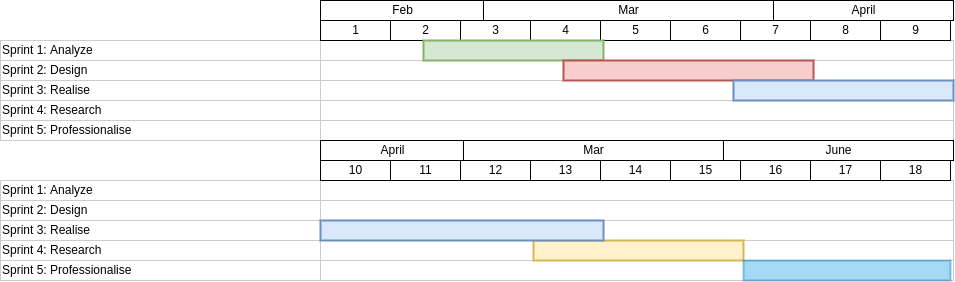
\includegraphics[width=1\textwidth]{ganttdiagram.png}
    \caption{Gantt Diagram Planning}
    \label{fig:ganttdiagram}
\end{figure}

The analyze sprint is expected to begin in the second half of the second week, when the project plan is finished and approved. Please note that there are 18 total weeks planned to work on the project, while there are 20 weeks of total resources planned. Two weeks (between 2/3 and 11/12) have been purposefully left out of the planning to be allocated at will. 

There is room to allocate more time in July if needed.

\section{Costs and Benefits}\label{costsandbenefits}
It is important to weigh the benefits against the costs. In this section, a complete overview is given of the expected benefits and the costs. As seen, while the initial costs of purchasing equipment might seem high


\begin{tabular}{ | l | l |}
    \hline
    \textbf{Subject} & \textbf{Costs} \\ \hline
    Professional Waterproof UAV & € 2.000 \\
    UAV Battery & € 250 \\
    UAV Controller & € 250 \\
    Various Sensors/Microcontrollers & € 300,- \\
    UAV Mounting hardware & € 100,- \\
    Proxy Shipping Service & € 100,- \\
    \hline
\end{tabular}


\subsection{Qualitative Benefits}
A few qualitative benefits are given:




\begin{itemize}
  \item \subsubsection*{Benefits} the benefits are very very clear
  \item The project must deliver every report described in project activities (\ref{interimresults}).
  \item The project must receive adequate funding as described in costs and benefits (\ref{costsandbenefits}).
  \item There must be accommodations to be able to test out the prototypes in the correct conditions.
\end{itemize}



Having more autonomous ways to monitor the water quality will lead to less man hours spent manually measuring the water. It will also allow for monitoring at places that aren't available yet.



\section{Risks}

\begin{figure}[h]
    \center
    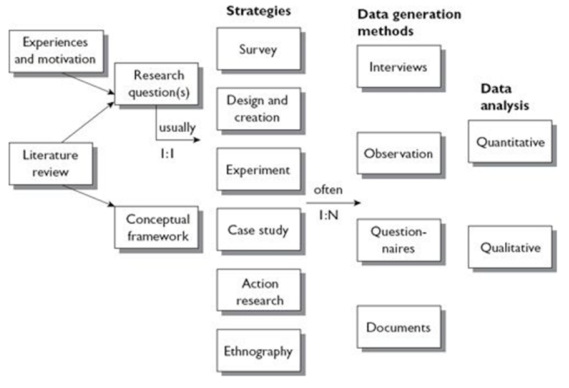
\includegraphics[width=0.5\textwidth]{research-strategies.png}
    \caption{Research strategies \cite{oates2005researching}}
    \label{fig:research_strategies}
\end{figure}

% References
\printbibliography 
\pagebreak
%Remove excerpt when publishing

\markdownInput{roelgrit.md}
\end{document}
